\documentclass{standalone}
\begin{document}

\chapter{Inertial Measurement Unit}
\label{Inertial Measurement Unit}
Inertial sensors, called Inertial Measurement Unit (\textbf{IMU}), is an electronic device of measurement that allows to estimate specific force, angular velocity and sometimes magnetic field of a body from the inertial forces that the body experiences. Its operation principle is based on the use and combination of forces from accelerometers, gyroscopes, and sometimes magnetometers\\
\noindent The inertial technology is based on the first two Newton’s laws. \\
\textit{The first law, affirms that the movement of a body is uniform and linear unless an external force is acting on it.} \\
\textit{The second law, defines that this force exerted on the mass will produce a proportional acceleration.
} 
\begin{center}
$ \textbf{F = ma} $
\end{center}

\noindent These relationships represent a \textit{measurement principle} from which can be developed sensing devices  able to measure the movement of bodies.
If we know the magnitude and direction of the forces applied to a body and its mass, we can know its acceleration. Speed and position are obtained from the acceleration versus time, by first and second mathematical integration.\\
Recent developments allow the production of IMU compatible with GPS devices. An IMU allows a GPS receiver to operate when GPS signals are not available, e.g. in tunnels, buildings or in the presence of electronic interference\cite{gpssystem} 
\newpage
\section{Operational Principles}\label{Operational Principles}
An IMU is a single unit into an electronics module which detects and collects angular velocity using one or more gyroscopes, linear acceleration data using one or more accelerometers and sometimes magnetic fields by using one or more magnetometer.\\
A typical configuration of IMU contains two separate sensors. \\First is the three-axial accelerometer. It 
generates three signals describing the accelerations along each of its axes. Second is the three-axial gyroscopes, it  outputs three analogue signals, and describe the vehicle angular velocity for each of the sensor axes.\\ Another possible configuration, contains also a three-axial magnetometer that produced three signal along each axis that describing the magnetic-field around the body.
\begin{center}
\begin{figure}[h]
\centering
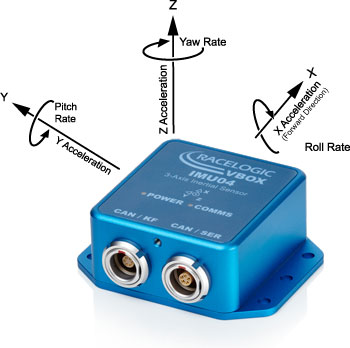
\includegraphics[scale=0.75]{imusensor}
\caption{Examples of IMU box.}
\label{fig:IMU box}
\end{figure}
\end{center}
\clearpage

\noindent The three axes around the sensors that produce the signals are \textbf{pitch}\footnote{The pitch axis (also called lateral axis) has its origin at the center of gravity and is directed to the right}, \textbf{roll}\footnote{The roll axis (or longitudinal axis) has its origin at the center of gravity and is directed forward}, and \textbf{yaw}\footnote{The yaw axis (Vertical axis) has its origin at the center of gravity and is directed towards the bottom of the vehicle}, in fact, IMUs works by detecting the changes in pitch, roll, and yaw.

\begin{center}
\begin{figure}[h]
\centering
\label{fig:Yaw Roll Pitch Frame of car}
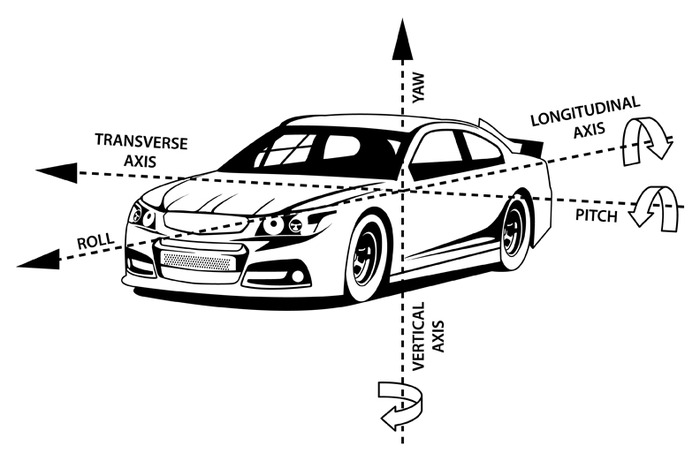
\includegraphics[scale=0.5]{yawpitchroll}
\caption{Frame of car respect Yaw, Pitch, and Roll Angle.}
\end{figure}
\end{center}
\clearpage	
	
	
\subsection{Uses}\label{IMU Uses}
\noindent Nowadays, IMU are often incorporated into Inertial Navigation Systems (INS), which use the raw IMU measurements, and after a processing and combination of these, is possible determine attitude, angular velocity, linear velocity and position relative to a global reference frame\footnote{a reference frame consists of an abstract coordinate system and the set of physical reference points that uniquely fix the coordinate system and standardize measurements.}, in our case the frame of the vehicle, as is shown in the Figure\ref{fig:Yaw Roll Pitch Frame of car}.\\ 
The IMU are highly applied for the navigation and control of the military, civil, and many commercial vehicles for real-time monitoring, and for geodetic navigation through post-processing of data.\\
Finding, ample space for use in space navigation systems, cars, ships, planes and aeroplanes.\\

The process to obtain velocity from acceleration and position from velocity, is known as dead reckoning. \footnote{The idea is to start from a known state (e.g. holding still) and calculate a new state (e.g. moving up or down) based on a measurement that indicates change, although it does not actually give you the info you want directly.}
In land vehicles, an IMU can be integrated into GPS based automotive navigation systems\footnote{An automotive navigation system is part of the automobile controls or a third party add-on used to find direction in an automobile. It typically uses a satellite navigation device to get its position data which is then correlated to a position on a road} or vehicle tracking systems\footnote{A vehicle tracking system combines the use of automatic vehicle location in individual vehicles with software that collects these data for a comprehensive picture of vehicle locations}, giving at the system a dead reckoning capability and the ability to gather as much accurate data as possible about the vehicle's current speed, turn rate, inclination and acceleration. \\
Besides navigational purposes, IMU serve as orientation sensors in many consumer products. Smartphones and Tablets contain IMU as orientation sensors. Fitness trackers and other wearable devices may also include IMU to measure motion.  They are a competing technology for use in motion capture technology\cite{motioncapture}.\clearpage
\section{Inertial Navigation System}\label{Inertial Navigation System}
An inertial navigation system (INS) is able to process the reported IMU data by a processor, like motion sensors (accelerometers) and rotation sensors (gyroscopes) to continuously calculate via dead reckoning the position, orientation, and velocity of a moving object without the need for external references\cite{basicprincipleaereo}.\\ 
The guidance system could show at pilot where the vehicle is located geographically at a certain moment, as with a GPS navigation system, but without the need to communicate with or receive communication from any outside components, such satellites. External sources are however used in order to correct drift errors.\\\\Recent advances in the construction of microelectromechanical systems (MEMS)\footnote{MEMS is the technology of microscopic devices, particularly those with moving parts.} have made the possibility to manufacture small and light inertial navigation systems, they are widely used in mobile devices, thanks to their small size without compromising performance.\\



\subsection{Principal Sensors}\label{Principal Sensors}
The main sensors of IMU system as we have discusses in the introduction\ref{Operational Principles} are the Accelerometer and Gyroscopes:
\begin{description}

\item [Accelerometer]: measure the linear acceleration of the moving vehicle in the sensor or body frame, but in directions that can only be measured relative to the moving system (the accelerometers are fixed to the system and rotate with the system, but are not aware of their own orientation). This can be thought as the ability of a blindfolded passenger in a car to feel themselves pressed back into their seat as the vehicle accelerates forward or pulled forward as it slows down; and feel themselves pressed down into their seat as the vehicle accelerates up a hill or rise up out of their seat as the car passes over the crest of a hill and begins to descend. Based on this information alone, they know how the vehicle is accelerating relative to itself, that is, whether it is accelerating forward, backward, left, right, up (toward the car's ceiling), or down (toward the car's floor) measured relative to the car, but not the direction relative to the Earth, since they did not know what direction the car was facing relative to the Earth when they felt the accelerations.
Note that the accelerometers will actually detect a force that is directed in the opposite direction from the
 acceleration vector. 
\item [Gyroscopes]: measure the angular velocity of the sensor frame with respect to the inertial reference frame. By using the original orientation of the system in the inertial reference frame as the initial condition and integrating the angular velocity, the system's current orientation is known at all times. This can be thought of as the ability of a blindfolded passenger in a car to feel the car turn left and right or tilt up and down as the car ascends or descends hills. Based on this information alone, the passenger knows what direction the car is facing but not how fast or slow it is moving, or whether it is sliding oblique.

\end{description}


\noindent An INS system is useful for a real-time monitoring but is possible getting the information about the velocity and position after processing IMU data when the travel is finished and the data are sent to a server or are stored into a device.


\section{Smartphone Sensors}\label{Smartphone Sensors}
Nowadays, smartphones are widely used in the world, and they are equipped with many sensors such as an accelerometer, gyroscope, touch-screen, ambient light sensor, proximity sensor, magnetometer, barometer, heart pulse rate monitor, for the purpose of this work the main sensor used is the accelerometer. Smartphone sensors are very cheap, and their size is getting smaller and smaller, in fact,they are also called Micro Electro-Mechanical-Systems (MEMS), motion sensors, and can offer great data results if compared with more both expensive and professional, so the information given by IMU is useful if the relations between the smartphone reference system, the vehicle reference system and the world reference system are known, in fact, by getting this information in real-time from the motion sensor is possible create an inertial navigation system by sensor data or process after the travel is finished if the data are stored, in fact there are many applications to allow the registration of the smartphone sensors data, it also be useful combine the use of the GPS.\\\\

\noindent These sensors are capable of providing raw data with high precision and accuracy, and are useful to monitoring three-dimensional device movement or positioning, or changes in the ambient environment near a device.\\\\
Usually a smartphone platform supports three broad categories of sensors:\cite{Andro}
\begin{itemize}
	\item Motion sensors: they measures acceleration forces and rotational forces along three axes. This category includes accelerometers, gravity sensors, gyroscopes, and rotational vector sensors.
	\item Environmental sensors: they measures various environmental parameters, such as ambient air temperature and pressure, illumination, and humidity. This category includes barometers, photometers, and thermometers.
	\item Position sensors: They measures the physical position of a device. This category includes orientation sensors and magnetometers.
\end{itemize}

\vspace{1cm}
\begin{figure}[ht]
\centering
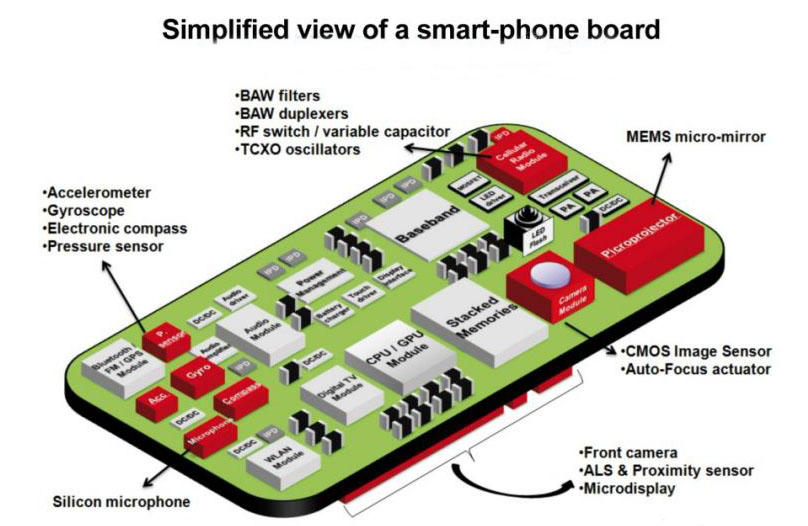
\includegraphics[scale=0.5]{sm_motherboard}
\caption{Sample view of the principals sensors inside smartphone}
\label{fig:Sample smartphone sensors}
\end{figure}


\paragraph{{\Large Accelerometer}}\leavevmode\\\\
Smartphones are builded with an accelerometer sensor.\\
They are sensitive to both linear acceleration and the local gravitational field, for each of the three-axes.\\ The accelerometer measures the acceleration of a smartphone against free fall, so allowing an application both determine the movement of the smartphone and its inclination.\\
The sensor consists of two components, a fixed and a mobile.\\
The second, moving according to the vibrations received, allows the first to measure and process the received data, then the distance variation between the capacitor\footnote{A capacitor is a passive two-terminal electrical component that stores electrical energy in an electric field.} armatures (so the electric capacity variation) will be used to determine the variation of the forces of acceleration which is subjected a device.\\ A special circuit records the variations created within the capacitor (these capacitors armatures are, made up of a moving mass and the fixed structure of the device) so that it can generate an electrical signal, proportional to the displacement of a mass.
The measurement is done for each axis ($x$, $y$, and $z$.), and it will be possible to measure the three-dimensional acceleration variation.\\The figure below\ref{fig:Sample smartphone accelerometer sensors} show the internal structure of accelerometer sensor.
\vspace{1cm}
\begin{figure}[h]
\centering
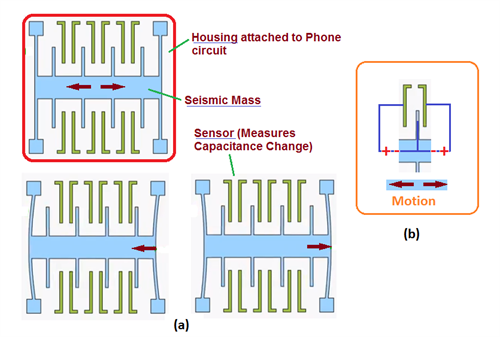
\includegraphics[scale=0.75]{smartphone-accelerometer}
\caption{Internal structure of smartphone accelerometer sensor}
\label{fig:Sample smartphone accelerometer sensors}
\end{figure}
\clearpage
\paragraph{{\Large Gyroscopes}}\leavevmode\\\\
The gyroscopes detects the current orientation of the device, or
changes in the orientation.\\ Orientation can be computed from the
angular velocity detected by the gyroscope, expressed in $rad/s$ on the three-axis.\\ 
A triple axis MEMS gyroscope, can measure rotation around the three axes: $x$, $y$, and $z$.
When the gyro is rotated, a small resonating mass is shifted as the angular velocity changes. This movement is converted into very low-current electrical signals that can be amplified and read by a host microcontroller.
The figure below show the internal structure of gyroscopes inside smartphone.


\vspace{1cm}
\begin{figure}[h]
\centering
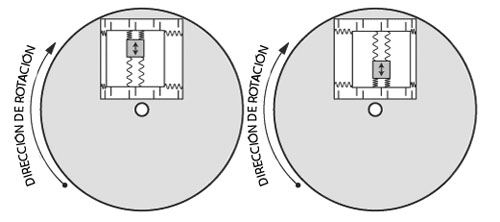
\includegraphics[scale=0.75]{Gyroscope-smartphone}
\caption{Internal structure of smartphone gyroscopes sensor}
\label{fig:Sample smartphone accelerometer sensors}
\end{figure}
\clearpage
\paragraph{{\Large GPS}}\leavevmode\\\\
All smartphones have GPS (Global Positioning System acronym), it is able to give our position. In good condition a GPS receiver indicates the location with an accuracy of about $10$ \si{\meter}. The aim of GPS system is to provide the coordinates of our position in terms of latitude, longitude and altitude.\\
The GPS system technically consists of 3 levels called segments:
\begin{description}
\item [Spatial Segment] is given by $31$ satellites rotating around the earth and which are the heart of GPS operation. The satellites travel to over $20.000$ \si{\km} from the ground.
\item [Control Segment] is provided by the main control station (and one of the reserve). The US military aircraft control satellites and carries out all related maintenance operations.
\item [User Segment] is simply the device with integrated GPS: navigator, smartphone, tablet, etc..
\end{description}

GPS can find our position on earth knowing:
\begin{itemize}
\item The distance from at least 3 satellites
\item The position of the satellites
\end{itemize}

The GPS receives the radio signal from the satellite that orbits in its vicinity and thanks to this signal, can calculate its distance using the simple formula:
\begin{center} $Distance = Time * Speed$ \end{center}

\noindent Speed: Satellite signal travels at speed of light ($299,792$ \si{\km\per\second})\\
Time: To find the time value, the satellite and the GPS of device (receveir) start from a common base signal, when the receiver has to calculate the position, receives from the satellite the signal, but having to travel thousands of kilometers the signal will come with a certain delay, this delay is the travel time were looking for. The signal usually arrived about in the order of $100ths$ of a second.
By multiplying the speed and travel time, our receiver will have distances from the satellites. To this end, the satellite sends the track of its position over time (which is stored in our device)

Once we have the exact distances from the satellite and its position, is possible find ours position on the earth. Triangulation technique is used for the purpose, through the information from the 3 satellites we solve a system of 3 equations with 3 unknowns: Latitude, Longitude and Altitude.\\
In general, the triangulation technique allows to find exactly our position as the intersection of three sphere having a radius equal to the distance of our point from the point of reference.\\\\
Actually, the intersection of the spheres produces two points in the space (one up and one down), but the problem is solved because considering the Earth sphere and inserting it into the geometric calculation we will have a single point on the earth surface representing our current position. As shown in the figure\ref{fig:Triangulation technique} below.
\vspace{1cm}
\begin{figure}[h]
\centering
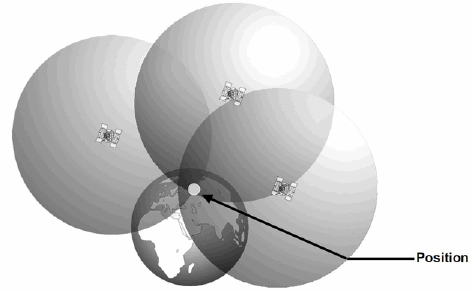
\includegraphics[scale=1]{Triangulation}
\caption{Triangulation technique}
\label{fig:Triangulation technique}
\end{figure}
\vspace{0.5cm}

There are 3 types of modes available on smartphones to get the GPS signal: 
\begin{itemize}
\item \textbf{High Accuracy}: uses data networks, Bluetooth, Wi-Fi or GPS to get the location
\item \textbf{Battery Saver}: uses data networks, Bluetooth or Wi-Fi to get the location
\item \textbf{Only Device}:  only uses the GPS sensor signal.
\end{itemize}

\noindent GPS works at $1$ $Hz$ once connection is established, thus the application records a sample of data once per second on average




\clearpage
\paragraph{{\Large Other Sensors}}\leavevmode\\\\
However, there are still many sensors available within smartphones, and they are:
\begin{description}
\item[Magnetometer]: detect magnetic fields. (compass applications use this to point at the planet's north pole)
\item[Proximity sensor]: it is placed near the earpiece of a phone. During a call, this sensor lets the system know that you're most probably in a call and that the screen has to be turned off.
\item[Light sensor]: measures how bright the ambient light is. The phone's software uses this data to adjust the display's brightness automatically.
\item[Barometer]: measures atmospheric pressure. Data measured by it is used to determine how high the device is above sea level, which in turn results in improved GPS accuracy. 
\item[Thermometer]: measures ambient temperature. Some handsets might have more than one of them(to monitor the temperature inside the device and its battery)
\item[Pedometer]: is a sensor used for counting the number of steps that the user has taken.
\item[Heart rate monitor]: measure one's pulse, and it does that by detecting the minute pulsations of the blood vessels inside one's finger.
\item[Fingerprint sensors]: the sensor is most convenient to use, as it does not require swiping in order to read fingerprint data.
\end{description}
\clearpage
\section{Error}\label{Error}
The major disadvantage of using IMU for navigation is that they typically suffer from accumulated error. Because the guidance system is continually integrating acceleration respect to the time to calculate velocity and position, any measurement errors, however small they are, are accumulated over time. This leads to \textit{"drift"}: an ever-increasing difference between where the system thinks it is located and the actual location. For the integration, a constant error in acceleration results in a linear error in velocity and a quadratic error growth in position.\cite{siciliano2016springer}\\
Signals from the IMU are processed by signal processing at a very high rate. For example, in a $100 Hz$ IMU, the sample period represents the total motion of the IMU over $10$ $ \si{milli\second}$. 
To reduce the effect of the measurement errors, they must be understood, estimated and then corrected
A well-designed system filter estimates and removes errors from the IMU measurements, reaching a higher attitude accuracy and longer solution stability .\\
The general error terms.
\begin{description}
\item [Repeatability]: the ability of the sensor to produce the same output for the same repeated input, assuming all other conditions are the same.
\item [Stability]: the ability of the sensor to produce the same output, over time, for the same constant input. 
\item [Drift]: the change of the output over time (zero drift is the change over time with no input).
\end{description}
Even when an IMU is stationary, it still measures forces. These measurements are the result of the IMU measuring forces in an inertial frame, a reference, fixed in space and time. Gravity acts in the inertial frame. The strong effect of gravity’s acceleration  can be measured by the accelerometers and is always significant when operating near the Earth’s surface.
Not all of these errors are relevant for all IMUs. Some of the error terms are too small to create a significant difference in the final solution. A key to having a high-performance processing system is to understand what the errors are in the system and developing ways to reduce or remove the errors and error sources, so a proper filter system needs to be developed, however during the integration the principal error is caused by the noise of the input IMU signal.



\end{document}

